\section{RCE Platform Hardware and Application to DUNE}
%%%%%%%%%%%%%%%%%%%%%%%%%%%%%%%%%%%%%%%%%%%%%%%%%%%%%%%%%%%%%%%%%%%%%
\subsection{RCE Overview}
\label{sec:RCEPlatformOverview}
%%%  Ryan

The core of the RCE platform is the Reconfigurable Cluster
Element (RCE), which is a system-on-chip design based upon
the Xilinx Zynq family of integrated circuits.
The RCE is a synergy of software and firmware. Together
they combine higher level programming with low level firmware
data processing, with a flexible boundary between the
two. An interface is defined at the software to firmware
boundary, defined here as the Protocol Plug In which provides 
a common API for both software to hardware and hardware to 
software interfaces. This interface is generic by design, 
assuring  that changes on either the hardware or software side 
of the interface do not impact the other.

\begin{figure}[tb]
\centering
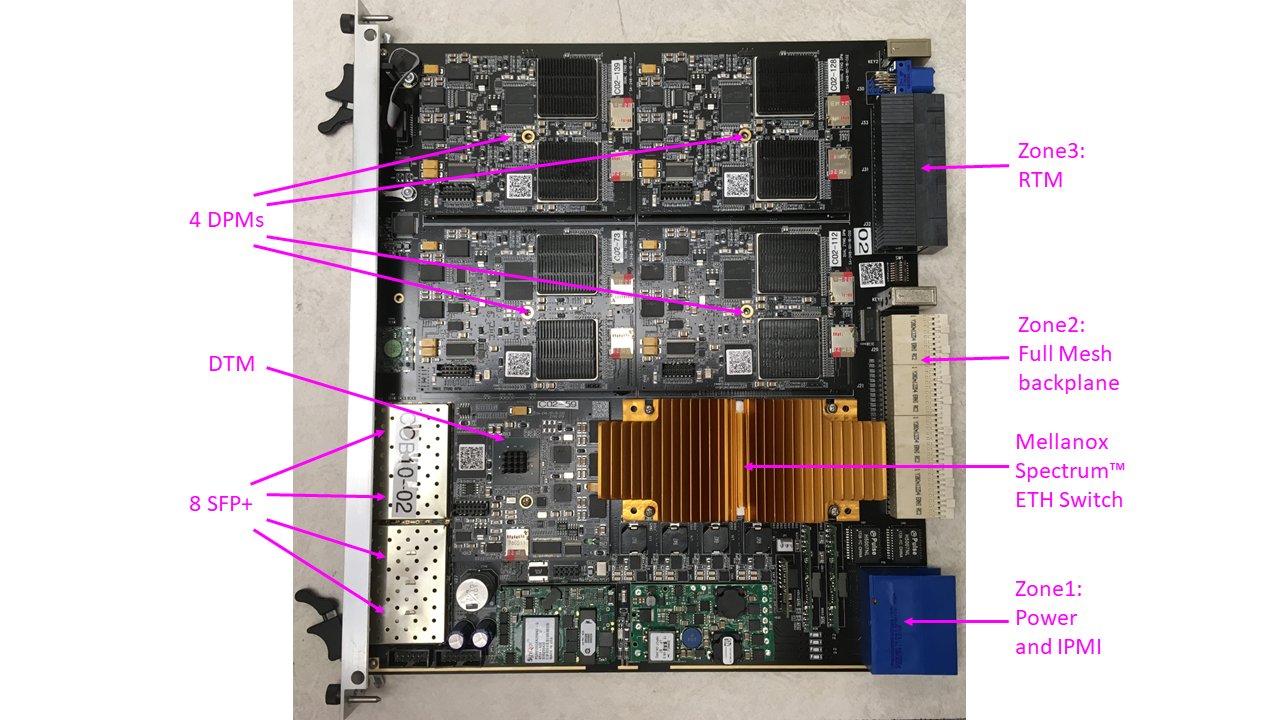
\includegraphics[width=0.9\textwidth]{images/COB_C10_pic_arrow.png}
\caption{\label{fig:COB_overview}COB Platform Overview}
\end{figure}

A set of RCE elements are hosted on a carrier board called the Cluster On Board (COB). This COB contains a local switch which provides 1Gbps, 10Gbps or 40Gbps links to up to 8 data processing RCE elements and 1 switch and timing control RCE. The data processing RCEs are hosted on 4 Data Processing Modules (DPMs) which support 1 or 2 RCEs. The Data Transport Module supports a smaller version of the RCE which is responsible for serving as the board timing hub as well as providing switch management functions. Each COB provides 3.2Tbps Ethernet switching capacity with maximum of 300ns latency between each RCE on a COB. 

\begin{figure}[tb]
\centering
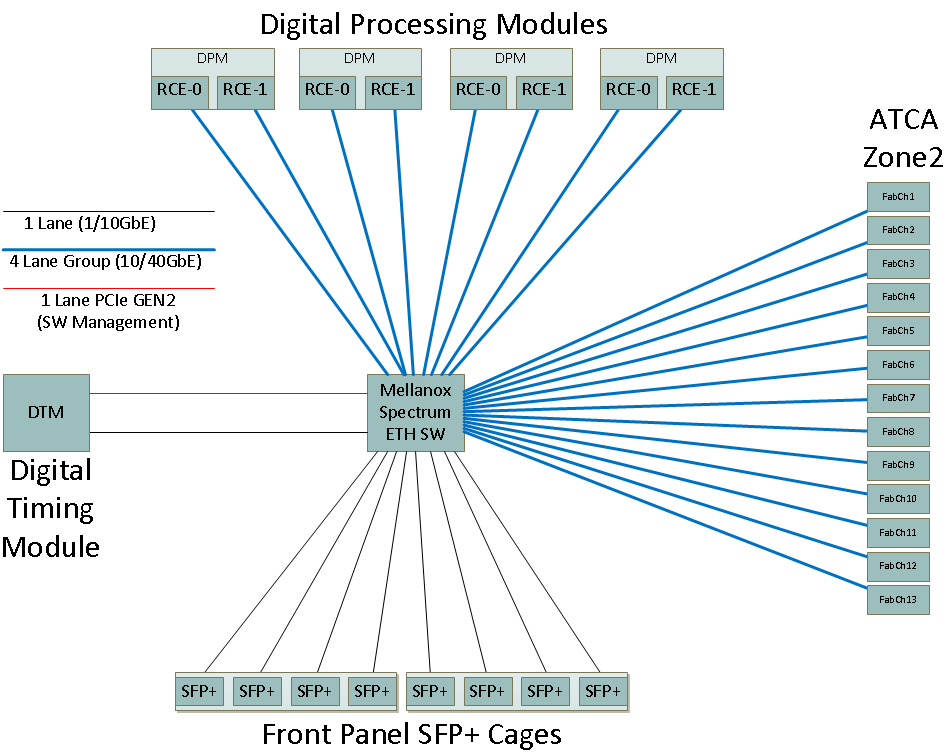
\includegraphics[width=0.9\textwidth]{images/COB_ETH-diagram.png}
\caption{\label{fig:COB_ETH_diagram}Block diagram of COB's Ethernet network}
\end{figure}

The COB also supports full mesh connectivity for a 14 slot ATCA crate. This allows up to 112 data processing RCEs to be fully interconnected with a total of 44.8Tbps of switching capacity with maximum of 600nS of latency between each of the 112 RCEs. Each COB also provides 80Gbps of external Ethernet connectivity, allowing multiple crates to be connected together to create large clusters of RCEs with a worst case latency of 1200nS between any two RCEs. This switching capacity also eliminates the need for an external Ethernet switch infrastructure. A single set of external links can be provided between the cluster and the back end processing system.

\begin{figure}[tb]
\centering
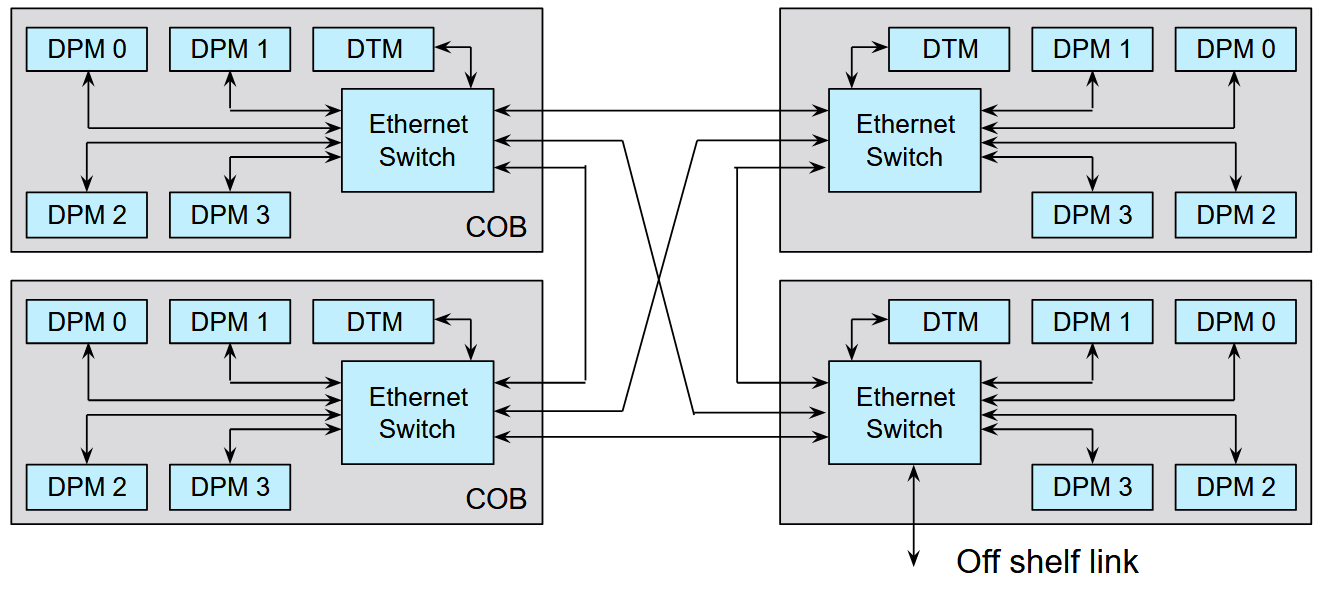
\includegraphics[width=0.9\textwidth]{images/RcePlatformClustering.png}
\caption{\label{fig:RcePlatformClustering}Block diagram of RCE Platform Clusting}
\end{figure}

The hardware side of this interfaces is designed around the AMBA 
bus standards (AXI4, AXI-Lite and 
AXI-Stream) which are supported by a large set of IP blocks 
provided by Xilinx and an extensive vendor independent firmware 
library created and maintained by the SLAC design team (SURF). Streaming data 
is moved in and out of processor memory using a high performance DMA 
engine provided as part of the SURF library. 

The software API utilizes a set of custom Linux kernel driver modules which 
provide access to both FPGA register space and streaming data to and from the 
DMA engine. The software API allows for zero copy DMA transactions to cachable user 
space buffers, utilizing the Xilinx ZYNQ ACP (accelerator coherency port). This 
streaming driver also allows reusing receive buffers for transmit data, allowing for 
received data to be received, buffered and transmitted out on demand without data copy
operations within software.

The RCE platform comes complete with a base set of firmware and software
which support both the core hardware and software functions of the platform, along with
providing the base interface between hardware and software. These modules include the 
software boot loader, the base kernel with its network and kernel drivers, the hardware
DMA engines, base registers, interrupt controller and networking support firmware. The platform
also includes a set of utilities for configuring and monitoring the RCE platform network
switch as well as full support for ATCA IPMI management and monitoring. More detail about this platform can be found in the 
2014 IEE NSS/MIC publication\cite{IEEE_RCE}.

%%%%%%%%%%%%%%%%%%%%%%%%%%%%%%%%%%%%%%%%%%%%%%%%%%%%%%%%%%%%%%%%%%%%%
\subsection{DUNE System Data Banwidths}
%%%  Larry

There are 2560 ADC channels per APA. For DUNE, we are planning to divide these channels evenly across 4 RCEs (640 channels per RCE).  The ADC values are 12-bit each and updated at 2 MHz, which makes the raw ADC data bandwidth to the RCE 15.36 Gb/s (1.92 GB/s).  Each RCE has a 8GB DRAM. We plan to dedicate 7 of the 8 GB for pre-buffering and the reset of the memory to the Linux kernel, DUNE runtime application and other misc. processes. To buffer 10 seconds into the 7 GB requires a real-time data compression factor of 3 (or better).  This data compression would be done in firmware (not software), which we have demonstrated in proto-DUNE and achieved a compression factor of 4.  With a data compression of 3, we would decrease the memory bandwidth into the pre-buffer to 5.12 Gb/s (0.64GB/s). 

As shown in refer Table \ref{tab:ComparingTechnicalSpecificsProcessorSide}, the raw memory bandwidth into the DRAM pre-buffer is 153.6 Gb/s (19.2GB/s).  When doing maximum data size bursting into DDR4 memory, writes are typically around 85\% efficient and reads are 70\% efficient.  For simplicity lets assume a worst-case scenario of 70\% for both types of operations, which reduce the DRAM pre-buffer bandwidth to 13.44GB/s.  When the super nova event happens pre-buffer will be doing both reads and write simultaneously into the pre-buffer, which we can assume the memory bandwidth requirement to be twice the compressed data rate (1.28GB/s). This means that we only need 9.5\% of the DRAM pre-buffer bandwidth to handle a super nova event. The software does have to share the DDR memory bandwidth with the super nova pre-buffer.  However, the DMA engine can configure the AXI memory interface to give any firmware DMA writes to the pre-buffer highest priority for the processor side's memory controller to mitigate the software from bottlenecking the pre-buffer's bandwidth.

The post-buffer SSD drive that we have selected is a Samsung NVMe 970 PRO, which is rated for write speeds up to 2.7GB/s and we have demonstrated 1.6GB/s into the Samsung NVMe SSD using ZYNQ Ultrascale+ (refer to Section \ref{sec:NVMe_Performance}).  Because the 1.6GB/s NVMe write speed is much greater than the targeted 0.64GB/s compressed data bandwidth, this Samsung NVMe solution meets the requirements of the post-buffering. With the smallest and cheapest Samsung NVMe 970 PRO drive of 512GB, we could store up to 800 seconds (8 supernova event post-buffers) at compression of 3 ratio. 

%%%%%%%%%%%%%%%%%%%%%%%%%%%%%%%%%%%%%%%%%%%%%%%%%%%%%%%%%%%%%%%%%%%%%
\subsection{The DUNE RCE and DPM}
%%%  Ryan

Figure \ref{fig:FW_block_diagram} depicts the data/timing/trigger flow of the RCE. The serial encoder timing stream is received and decoded on each RCE.  The recovered clock from the timing serial stream is used to run each RCE synchronous to each other. The ADC data is received over the WIB links (total of 4 WIB links per RCE). The raw ADC from the WIB links is sent to trigger primitive and data compression firmware modules. The trigger primitive firmware module does feature extraction of the waveforms to generate a trigger primitive message.  The data compression firmware compresses the data volume for the pre-buffer DRAM ring buffer. The processor side (which standard Linux software runs) controls the pre/post buffer management and trigger controls.  The software uses TCP communication for slow controls/monitoring, trigger messaging and data flow. 

\begin{figure}[tb]
\centering
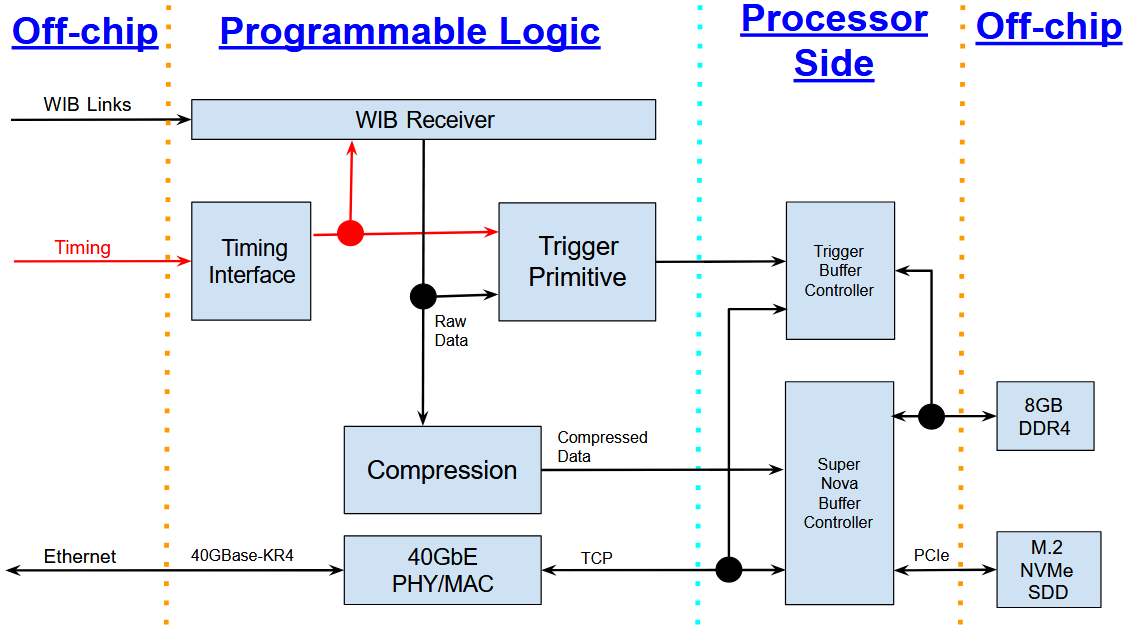
\includegraphics[width=0.9\textwidth]{images/FW_block_diagram.png}
\caption{\label{fig:FW_block_diagram}DAQ concept showing the SN system as well as the trigger primitive and full data stream.}
\end{figure}

%%%%%%%%%%%%%%%%%%%%%%%%%%%%%%%%%%%%%%%%%%%%%%%%%%%%%%%%%%%%%%%%%%%%%
\subsubsection{Migrating the DPM design from ZYNQ-7000 to ZYNQ Ultrascale+ for DUNE}
%%%  Larry

\begin{figure}[tb]
\centering
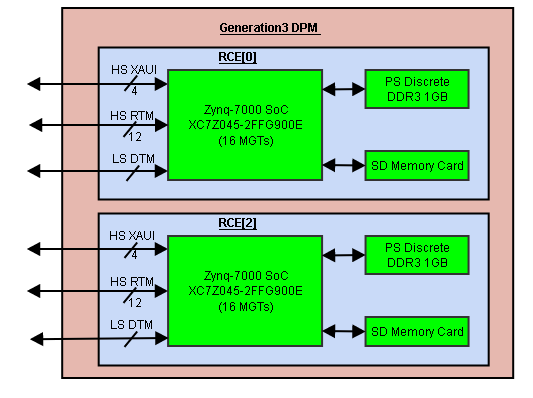
\includegraphics[width=0.5\textwidth]{images/proto-dune-dpm.png}
\caption{\label{fig:proto-dune-dpm} Block diagram of the proto-DUNE DPM}
\end{figure}

The DPM design used for proto-DUNE and designed by SLAC was based on a ZYNQ-7000 architecture. A block diagram of this proto-DUNE DPM is shown in Figure \ref{fig:proto-dune-dpm}.  While we were successfully able to use this DPM design for proto-DUNE (256 channels per RCE and no NVMe post-buffering), the increasing of the ADC channel count for DUNE prevents us from reusing this existing design due to the increased memory bandwidth requirements on the pre-buffer DRAM.  Another limitation of the proto-DUNE DPM 800MHz dual CPU was not powerful enough to do anything but move zero-copy buffers around from the DPM and simple slow controls/monitoring. We even had to bypass the software TCP and implemented a reliable UDP (RDUP) in firmware to offload the CPU load to keep up with the proto-DUNE trigger rate.  

To address these issues, we have done a design study of the next generation ZYNQ called "ZYNQ Ultrascale+" as a possible upgrade path. Tables of comparing technical specifications between the ZYNQ-7000 to ZYNQ Ultrascale+.   As shown in the Table \ref{tab:ComparingTechnicalSpecificsProcessorSide}, we can expect about a factor of 4 DRAM memory bandwidth improvement, which is greater than our 2.5 factor increase of ADC channels per RCE.  The signification improvements in the processing side (from 32-bit CPU to 64-bit, increase in CPU cores/speed, additional dual Realtime CPU and additional GPU) opens up the possibility to have the software be more involved in the DAQ, which was a limitation in proto-DUNE DPM.

\begin{table}[tb]
\centering
\scalebox{0.75}{
\begin{tabular}{|c|c|c|c|c|c|c|c|c|c|c|c|}
\hline
\multirow{2}{*}{} & \multicolumn{2}{c|}{Application CPU} & \multicolumn{2}{c|}{Real-time CPU} & \multicolumn{2}{c|}{GPU} & \multicolumn{5}{c|}{DRAM} \\ \cline{2-12} 
 & \# cores & Freq. & \# cores & Freq. & \# cores & Freq. & Type & Size & Width & Speed & \begin{tabular}[c]{@{}c@{}}Raw Peak \\ Bandwidth\end{tabular} \\ \hline
\begin{tabular}[c]{@{}c@{}}proto-DUNE DPM\\ (XC7Z045-2FFG900E)\end{tabular} & 2 & 0.8GHz & 0 & N/A & 0 & N/A & DDR3 & 1GB & 32-bit & 1.066Gb/s & 34Gb/s \\ \hline
\begin{tabular}[c]{@{}c@{}}DUNE-DPM\\ (XCZU15EG-1FFVC900E)\end{tabular} & 4 & 1.2GHz & 2 & 0.5GHz & 2 & 0.6GHz & DDR4 & 8GB & 64-bit & 2.4Gb/s & 153.6Gb/s \\ \hline
\end{tabular}}
\caption{Comparing Technical Specifications of the Processor Side}
\label{tab:ComparingTechnicalSpecificsProcessorSide}
\end{table}

\begin{table}[tb]
\centering
\begin{tabular}{|c|c|c|c|c|c|}
\hline
 & kLUTs & kFFs & BRAM & URAM & DSP48 \\ \hline
\begin{tabular}[c]{@{}c@{}}proto-DUNE DPM\\ (XC7Z045-2FFG900E)\end{tabular} & 218 & 437.2 & 19.2Mb & 0Mb & 900 \\ \hline
\begin{tabular}[c]{@{}c@{}}DUNE-DPM\\ (XCZU15EG-1FFVC900E)\end{tabular} & 341 & 683 & 26.2Mb & 31.5Mb & 3,528 \\ \hline
\end{tabular}
\caption{ Comparing Technical Specifications of the Programmable Logic Side}
\label{tab:ComparingTechnicalSpecificsProgrammableLogicSide}
\end{table}

\begin{figure}[tb]
\centering
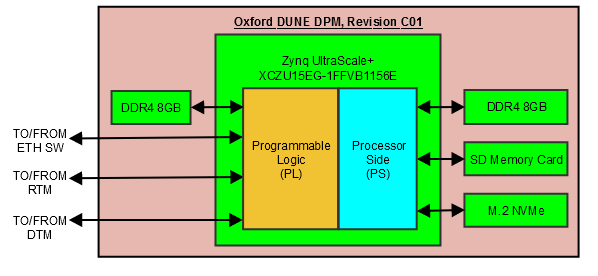
\includegraphics[width=0.8\textwidth]{images/OxfordBlockDiagram.png}
\caption{\label{fig:OxfordBlockDiagram} Block diagram of the Oxford/SLAC DPM being used for double buffering proof of concept}
\end{figure}

Oxford and SLAC has been collaborating on a ZYNQ Ultrascale+ DPM design for "proof of concept" of double buffering.  DPM design for DUNE. A block diagram of this Oxford/SLAC DPM is shown in Figure \ref{fig:OxfordBlockDiagram}. On the processor side is a 8GB of DRAM and a M.2 NMVe interface.  On the programmable logic side is all the electrical interfaces to the COB ETH switch, RTM and DTM plus an optional 8GB DRAM.

\begin{figure}[tb]
\centering
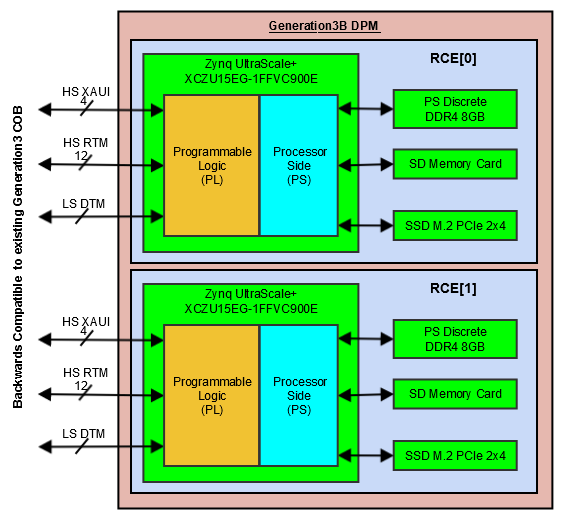
\includegraphics[width=0.9\textwidth]{images/DpmUltrascaleBlockDiagram.png}
\caption{\label{fig:DpmUltrascaleBlockDiagram} Block diagram of proposed dual Zynq Ultrascale+ design for DUNE}
\end{figure}

While the proto-DUNE DPM had two RCE elements per DPM, this proof of concept DPM is only one RCE element per DPM.  The disadvantage of halfing the DPM's RCE density is that the RTM, COB and ATCA crate cost crates are doubled. We are proposing a dual ZYNQ Ultrascale+ DPM design for DUNE that has all the features and interfaces of the Oxford/SLAC DPM minus the optional 8GB DRAM (due to board layout constraints). A block diagram of this proposed DPM design is shown in Figure \ref{fig:DpmUltrascaleBlockDiagram}.  This would make the RCE platform 2 APAs per COB (instead of 1 APA per COB). Because we are only replicating the Oxford/SLAC electrical circuits twice on a DPM, all firmware/software development using the Oxford/SLAC can be reused with little to no additional effort. 

%%%%%%%%%%%%%%%%%%%%%%%%%%%%%%%%%%%%%%%%%%%%%%%%%%%%%%%%%%%%%%%%%%%%%
\subsection{NVMe Performance}
\label{sec:NVMe_Performance}
%%%  Larry

To benchmark the ZYNQ Ultrascale+'s post-buffer write performance, we ran ArchLinux on the Xilinx ZCU102 development board doing 100GB bursting with EXT4 filesystem on the SSD.  With a M.2 NVMe to PCIe card adapter, we were able to connect the Samsung SSD drive to the ZYNQ's processor PCIe interface.  A photograph of this test setup is shown in Figure \ref{fig:NMVe_performance}. We were only able to achieve 1.6GB/s file write speeds.  This Samsung 960 PRO\cite{Datasheet}(Samsung 970 PRO not available at this time of measurement) is rate for 2.1 GB/s write speeds.  However, the ZYNQ Ultrascale+ is only 4 lanes for PCIe Generation 2 (not Generation 3).  The theoretical link bandwidth limit (serial rate) of PCIe Generation 2 and 4 lanes is 2.0GB/s.  We are assuming that the 1.6GB/s is due to the inefficiency of the PCIe data packets. 

\begin{figure}[tb]
\centering
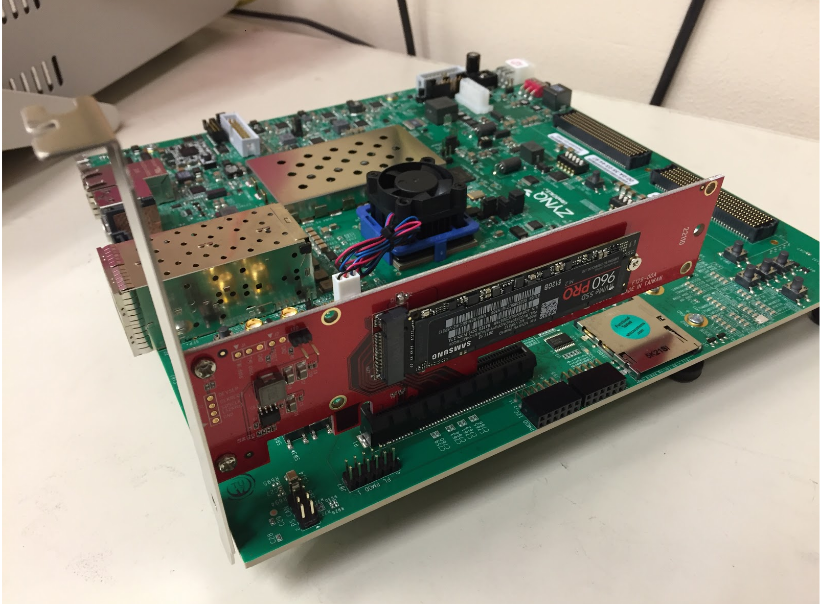
\includegraphics[width=0.5\textwidth]{images/NMVe_performance.png}
\caption{\label{fig:NMVe_performance} Photograph of the ZCU102 development board and Samsung NVMe SSD 960 PRO}
\end{figure}

%%%%%%%%%%%%%%%%%%%%%%%%%%%%%%%%%%%%%%%%%%%%%%%%%%%%%%%%%%%%%%%%%%%%%
\subsection{The DTM and timing distribution}
%%%  Larry

The DTM receives the timing serial stream from the RTM's SFP timing interface.
This timing serial stream is repeated to each of the RCEs within a COB. 
For standalone mode (when a timing serial stream is not available), the 
DTM can multiplex a emulated time serial stream to the RCEs. 

%%%%%%%%%%%%%%%%%%%%%%%%%%%%%%%%%%%%%%%%%%%%%%%%%%%%%%%%%%%%%%%%%%%%%
\subsection{The RTM}
%%%  Larry

\begin{figure}[tb]
\centering
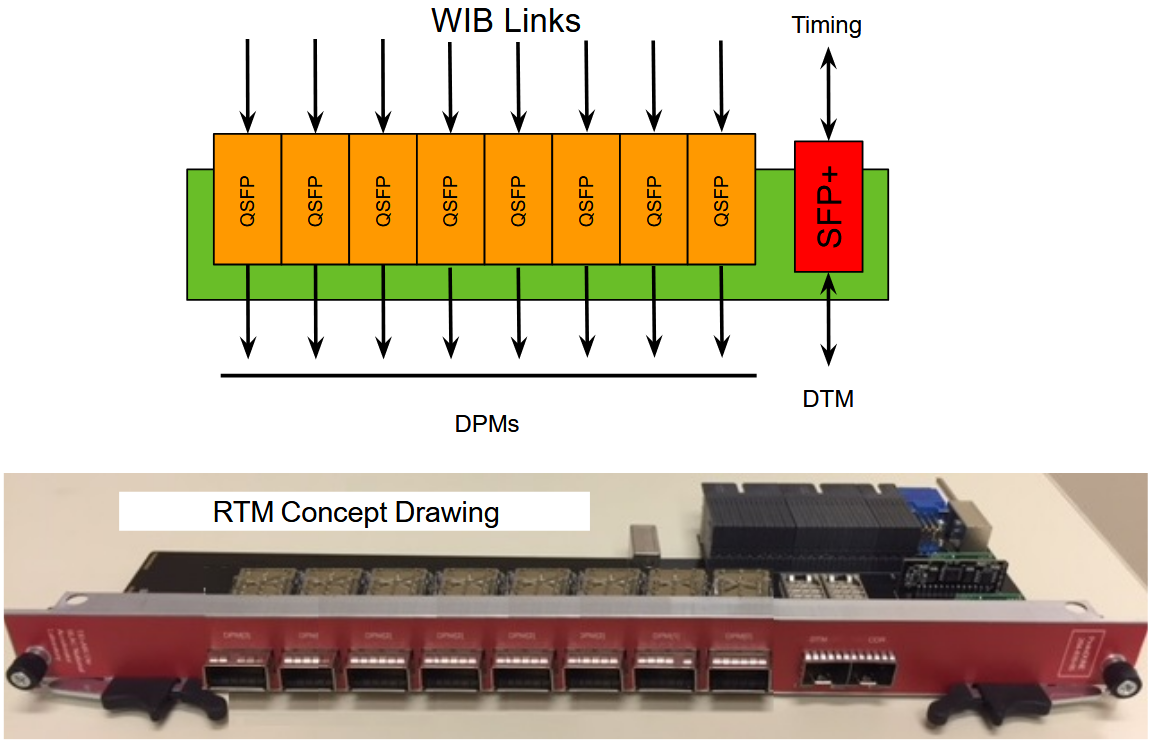
\includegraphics[width=0.5\textwidth]{images/RTM_block_diagram.png}
\caption{\label{fig:RTM_block_diagram}Block diagram and concept art of the DUNE RTM.}
\end{figure}

A block diagram of the Rear Transition Module (RTM) is shown in Figure \ref{fig:RTM_block_diagram}. This RTM has 8 QSFP fiber optic cages (4 fiber links per RCE element), which adds up to a total of 32 fiber links per APA.  Each fiber link needs to transport 4Gb/s of data.  The QSFP form factor was select due to its high fiber count and very cheap optics (commonly used in telecomm 40 Gb/s Ethernet optical networks). An additional SFP+ cage is required to interface to the timing system. 

This board is basically a "passive" optical-to-electrical converter (no firmware or software required).  The simplicity of this board design helps keep the cost down for the DAQ system. 

%%%%%%%%%%%%%%%%%%%%%%%%%%%%%%%%%%%%%%%%%%%%%%%%%%%%%%%%%%%%%%%%%%%%%
\subsection{ATCA Rack Space Estimates}
%%%  Larry

Assuming that we use the dual Zynq Ultrascale+ solution per DPM, there would be 2 APAs per COB (640 ADC channels per RCE). This means we would be able to fit the entire experiment of 150 APAs into 75 COBs.  If we are using 14-slot ATCA crates, it would only take 6 ATCA crate for all 150 APAs. 14-slot ATCA crates are available in 15U rack space. Assuming a standard 42U rack, it would only require 3 racks for the entire experiment of 150 APAs (2 ATCA crates per rack). Because of the limited rack space underground for DUNE, having a min. rack space footprint is important.

%%%%%%%%%%%%%%%%%%%%%%%%%%%%%%%%%%%%%%%%%%%%%%%%%%%%%%%%%%%%%%%%%%%%%
\subsection{ATCA Power/Cooling Estimates}
%%%  Larry

The maximum possible power per COB is 300W (limited ATCA cooling capability per slot).  For worst-case scenario assume that each COB will be 300W in operation, which would add up to 22.5 kW (=300W/COB * 75 COBs).  Lets also assume that the auxiliary ATCA electronics (shelf manager and fans) take about 250W per crate, which would add up to 1.5 kW (=250W/crate * 6 crates). Then the total power/cooling requirement for the ATCA electronics would be 24 kW.  Because of the limited cooling and limited electrical AC power capability of the underground space for DUNE, having a min. power/cooling footprint is important as well. 

%%%%%%%%%%%%%%%%%%%%%%%%%%%%%%%%%%%%%%%%%%%%%%%%%%%%%%%%%%%%%%%%%%%%%
\subsection{ ATCA Shelf Manager and IPMI}
%%%  Ryan

ATCA is a telecom standard designed for “5 nines” uptime.
Almost all components can be replaced in the field.
Redundancy is available if desired but not required.
The shelf manager provides the IPMI interface to all components in the crate. 
Shelf manager generates alarms when warning or error events occur
(Example: electronics overheating). 

\begin{figure}[tb]
\centering
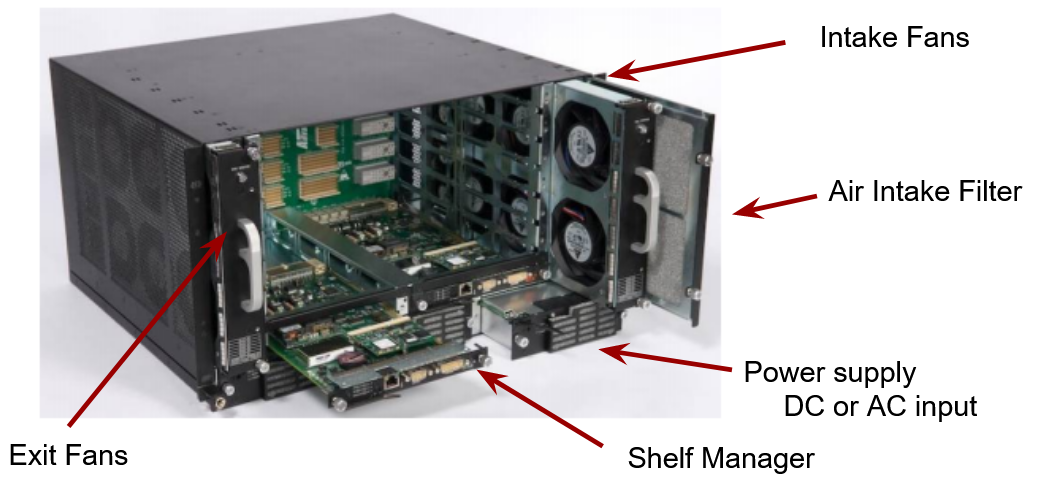
\includegraphics[width=0.5\textwidth]{images/ATCA_Components.png}
\caption{\label{fig:ATCA_Components}Diagram of the ATCA components}
\end{figure}

%%%%%%%%%%%%%%%%%%%%%%%%%%%%%%%%%%%%%%%%%%%%%%%%%%%%%%%%%%%%%%%%%%%%%